\title{Study Guide for Midterm 2}
\author{Dr. Jordan Hanson - Whittier College Dept. of Physics and Astronomy}
\date{\today}
\documentclass[10pt]{article}
\usepackage[a4paper, total={18cm, 27cm}]{geometry}
\usepackage{outlines}
\usepackage{graphicx}
\begin{document}
\maketitle

\section{Chapter 6 - Functions of Combinational Logic}
\label{sec:comb2}

\begin{enumerate}
\item a) Design a circuit below that adds two numbers in binary corresponding to outputs from two separate encoders. (b) Demonstrate how your design would add 1 and 9 with a timing diagram.  (c) Add a separate input line with XNOR gates that switches the system to subtraction in 2's complement form. \\ \vspace{3.5cm}
\item Using basic logic gates like XNOR, AND, and inverters, (a) create a comparator that yields HIGH if the \textit{magnitude} of two 2-bit binary numbers is equal.  Assume that one or both of the numbers is a negative one, and that if a number is negative it is in \textit{1's complement form.} \\ \vspace{3.5cm}
\item Generate the logic gates that convert 4-bit binary to 4-bit gray code, and show that it works with a timing diagram. \\ \vspace{2cm}
\item Consider Fig. \ref{fig:par}. (a) Produce the output timing diagram.  (b) Now develop a symbol for the 4 parallel bit parity checker, and connect four of them to a 4-to-1 multiplexer, with two data select lines. (c) Devise a \textit{simple} timing diagram that align the data select lines with parity check outputs.
\begin{figure}[hb]
\centering
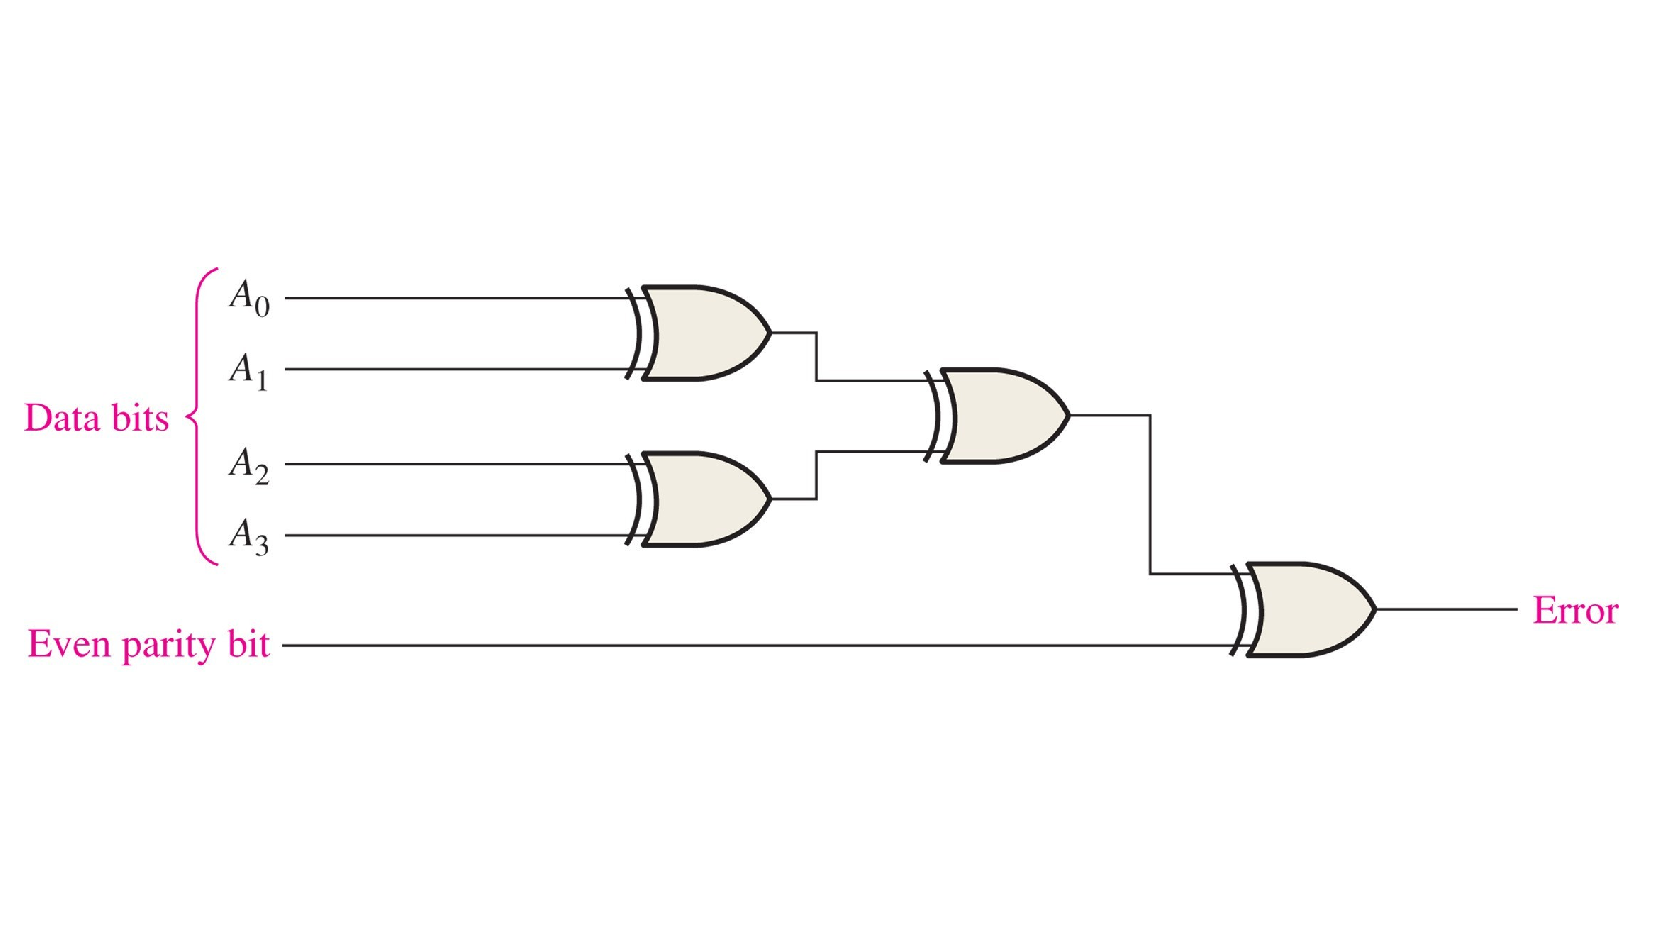
\includegraphics[width=0.55\textwidth]{figures/parityCheck.pdf}
\caption{\label{fig:par} A parity checker for 4 parallel bits.}
\end{figure}
\end{enumerate}

\clearpage

\section{Chapter 7 - Latches, Flip-flops, and Timers}
\label{sec:latch}
\begin{enumerate}
\item Consider Fig. \ref{fig:detect}.  (a) If the CLK signal frequency is 20 MHz, what is the period? (b) If the delay through the inverter is 5 ns, what is the pulse width of the output from the pulse transition detector? (c) What is the duty cycle relative to the CLK signal? (d) Produce the timing diagram of the D-FF with the following bitstream as the input: $10001000$, where each new bit is associated with a CLK pulse.
\begin{figure}[ht]
\centering
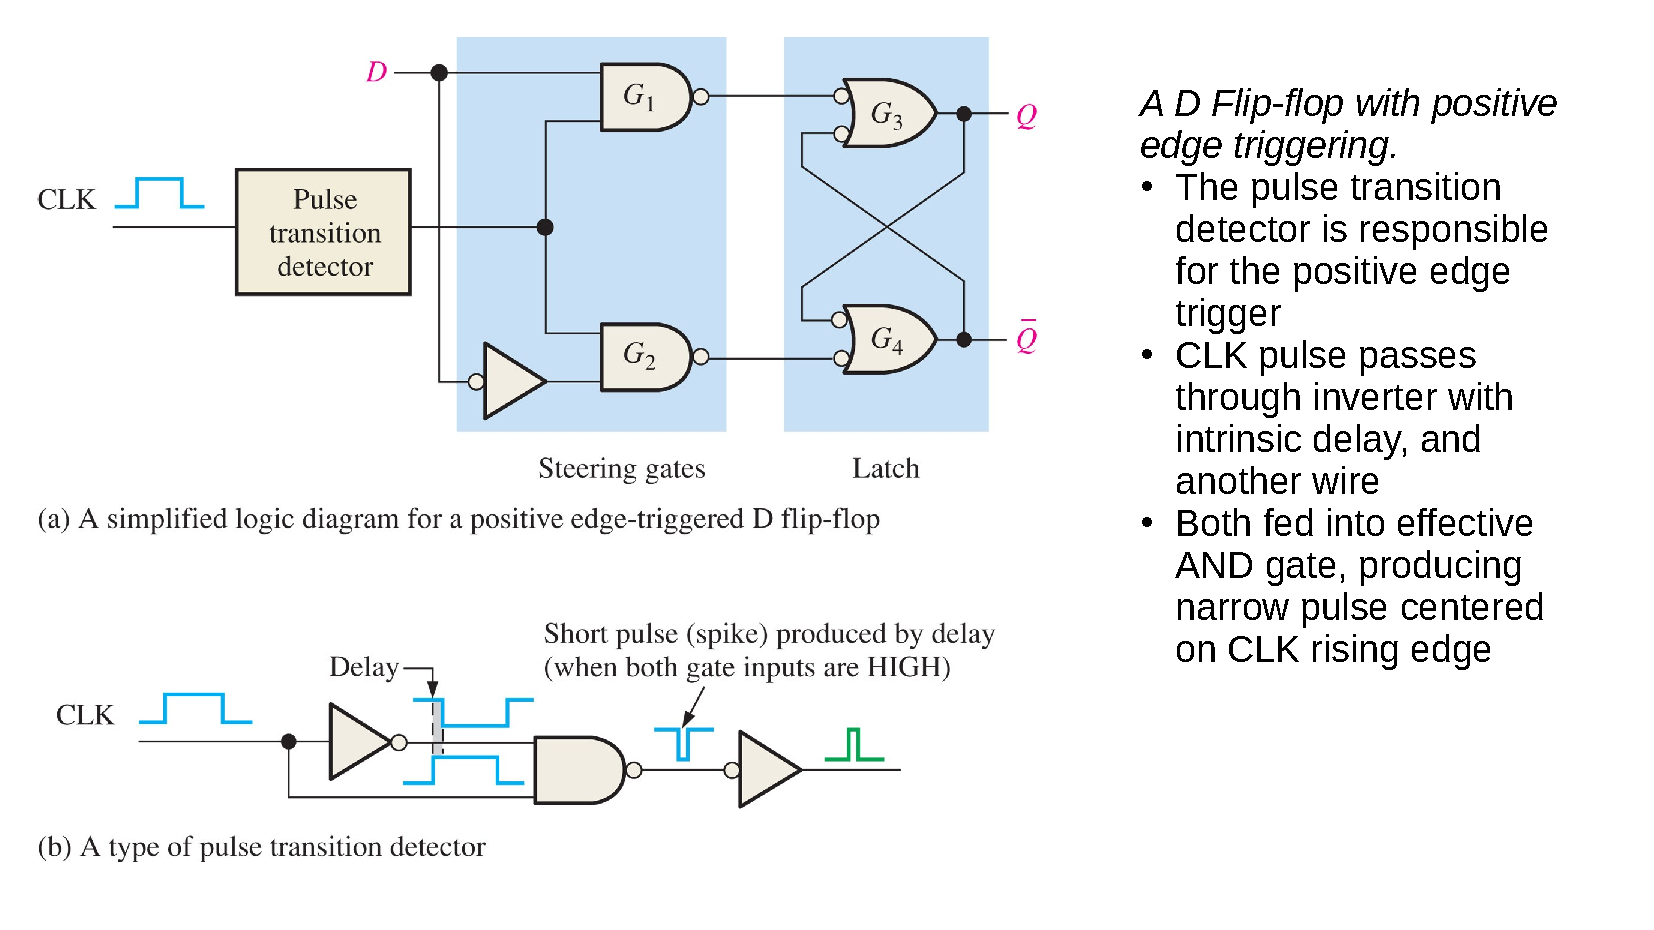
\includegraphics[width=0.75\textwidth]{figures/detect.pdf}
\caption{\label{fig:detect} The inner workings of a D FF with positive edge trigger.}
\end{figure}
\item Consider Fig. \ref{fig:detect2}. (a) If the CLK frequency is 40 MHz, with what frequency does the $Q$ output oscillate? (b) Using the same principle, construct a circuit with JK flip-flops that changes the CLK frequency from 40 MHz to 10 MHz.
\begin{figure}[hb]
\centering
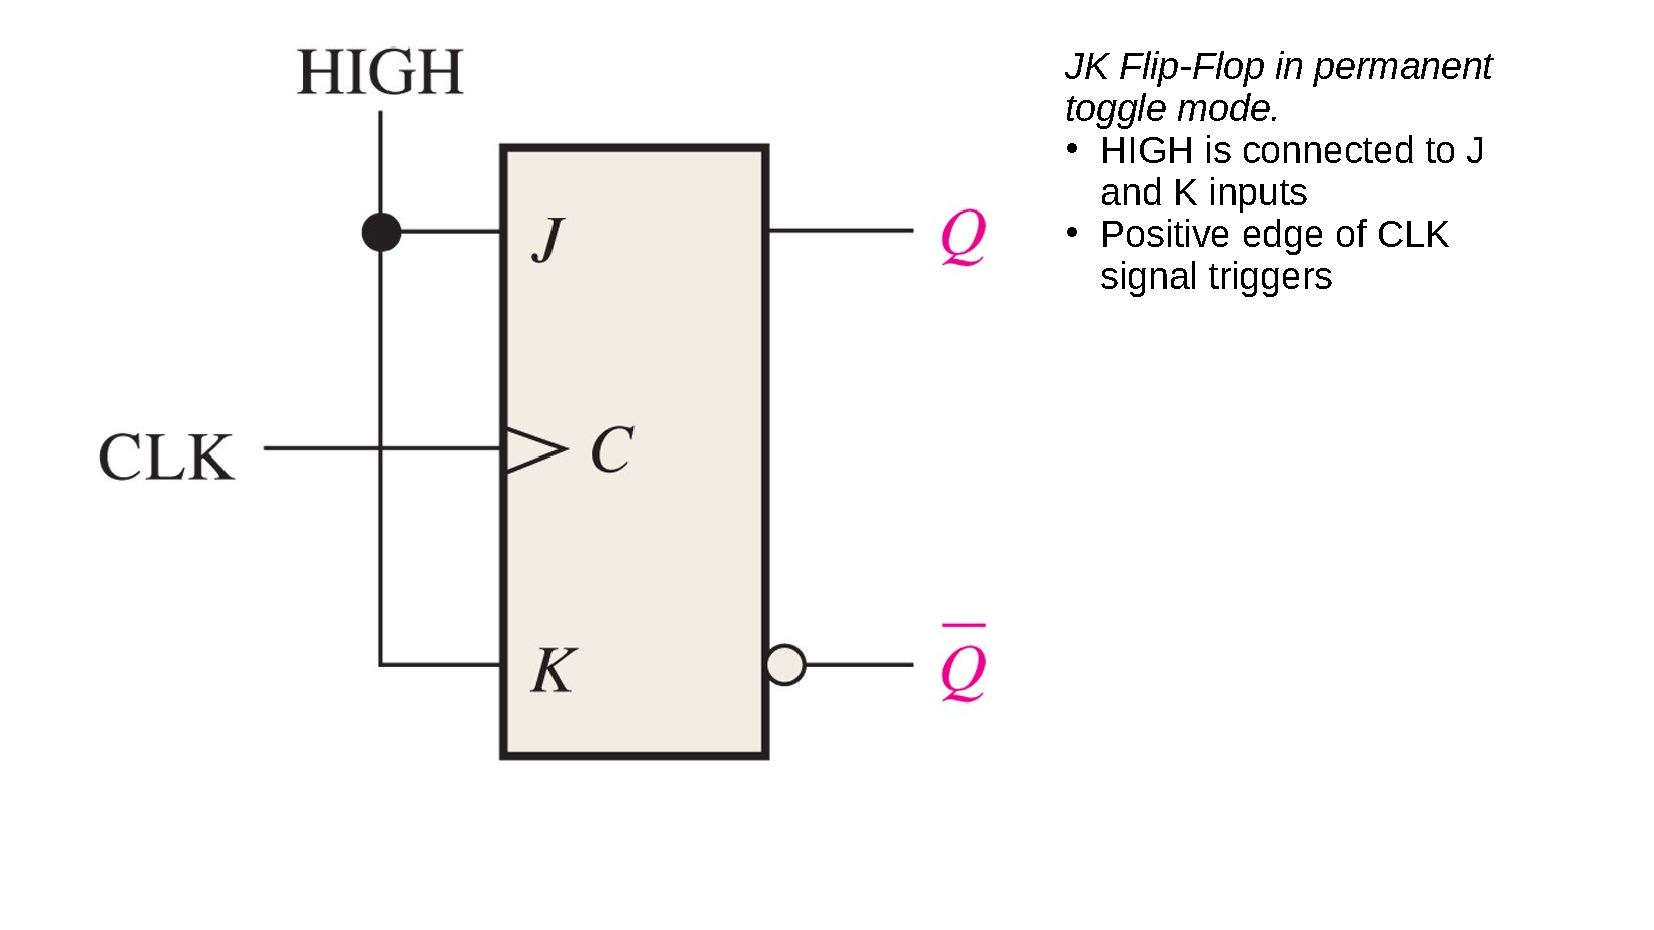
\includegraphics[width=0.5\textwidth]{figures/detect2.pdf}
\caption{\label{fig:detect2} A simple circuit built from a JK flip-flop (FF).}
\end{figure}
\end{enumerate}

\clearpage

\section{Chapters 8 and 9 - Shift Registers and Counters}

\begin{enumerate}
\item Consider Fig. \ref{fig:sr1}.  (a) Design a timing diagram and serial input (serial data in) that causes a single bit to enter the register and then bounce from right to left repeatedly. (b) What is the frequency and duty cycle of $Q_3$?
\begin{figure}[ht]
\centering
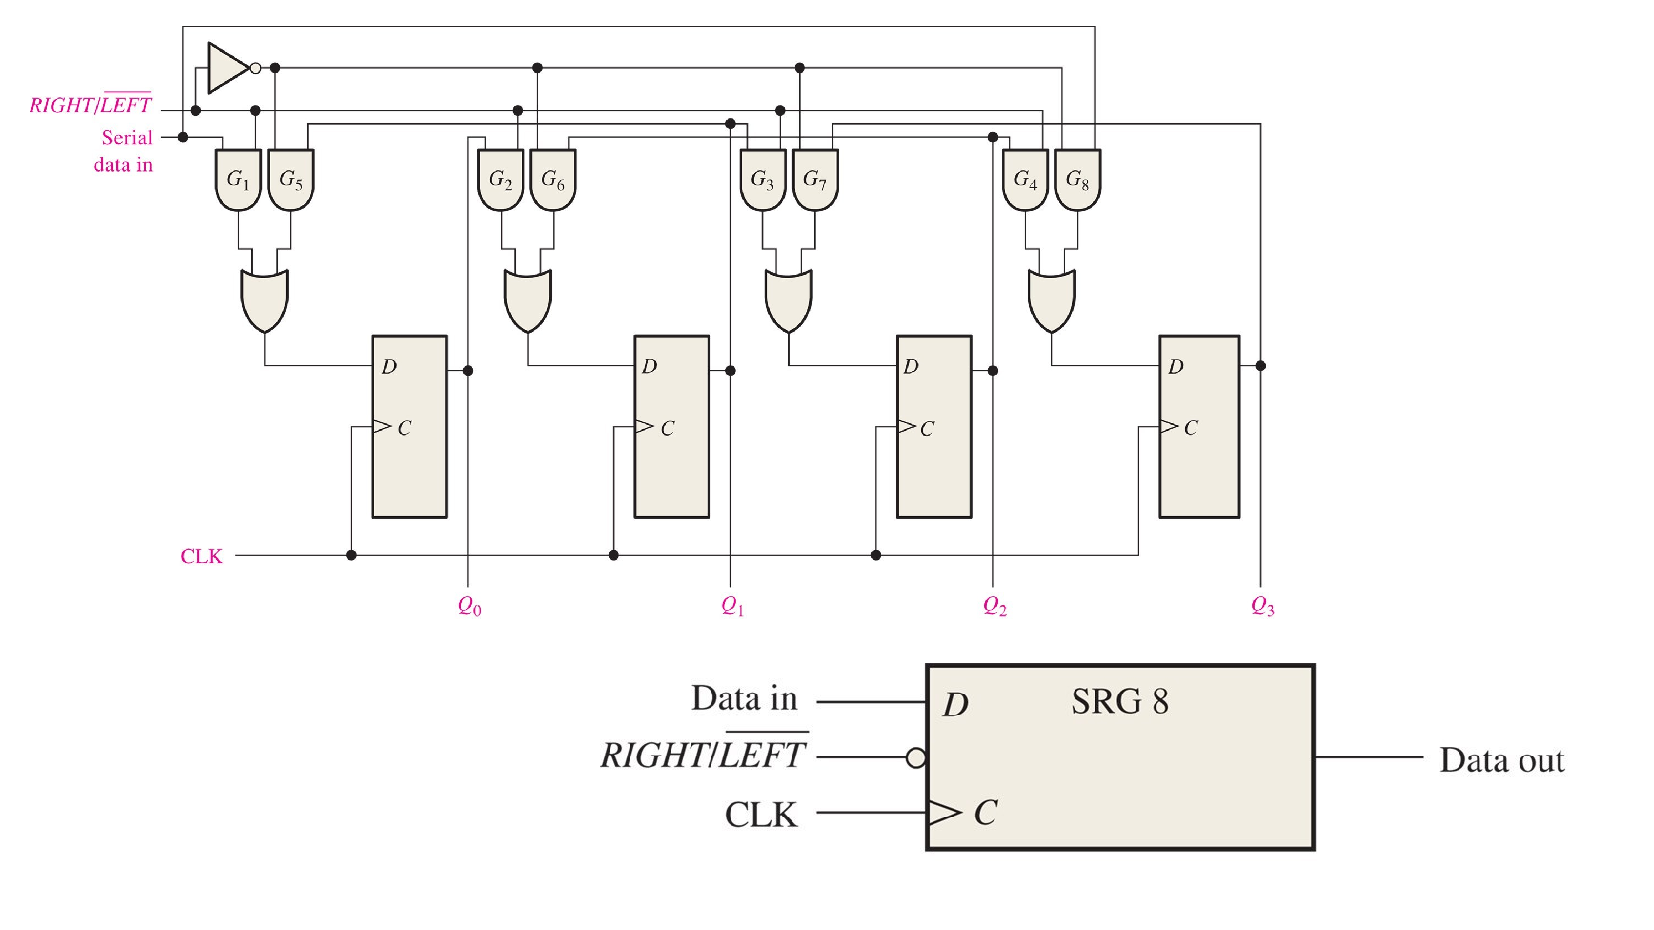
\includegraphics[width=0.8\textwidth,trim=0cm 5cm 0cm 0cm,clip=true]{figures/shift_register1.pdf}
\caption{\label{fig:sr1} A 4-bit bidirectional shift register.}
\end{figure} \vspace{4cm}
\item Consider Fig. \ref{fig:count}.  The waveforms are applied to the count enable, clear, and clock inputs as indicated.  Show the counter output waveforms in proper relation to these inputs.  The clear input is asynchronous.
\begin{figure}[hb]
\centering
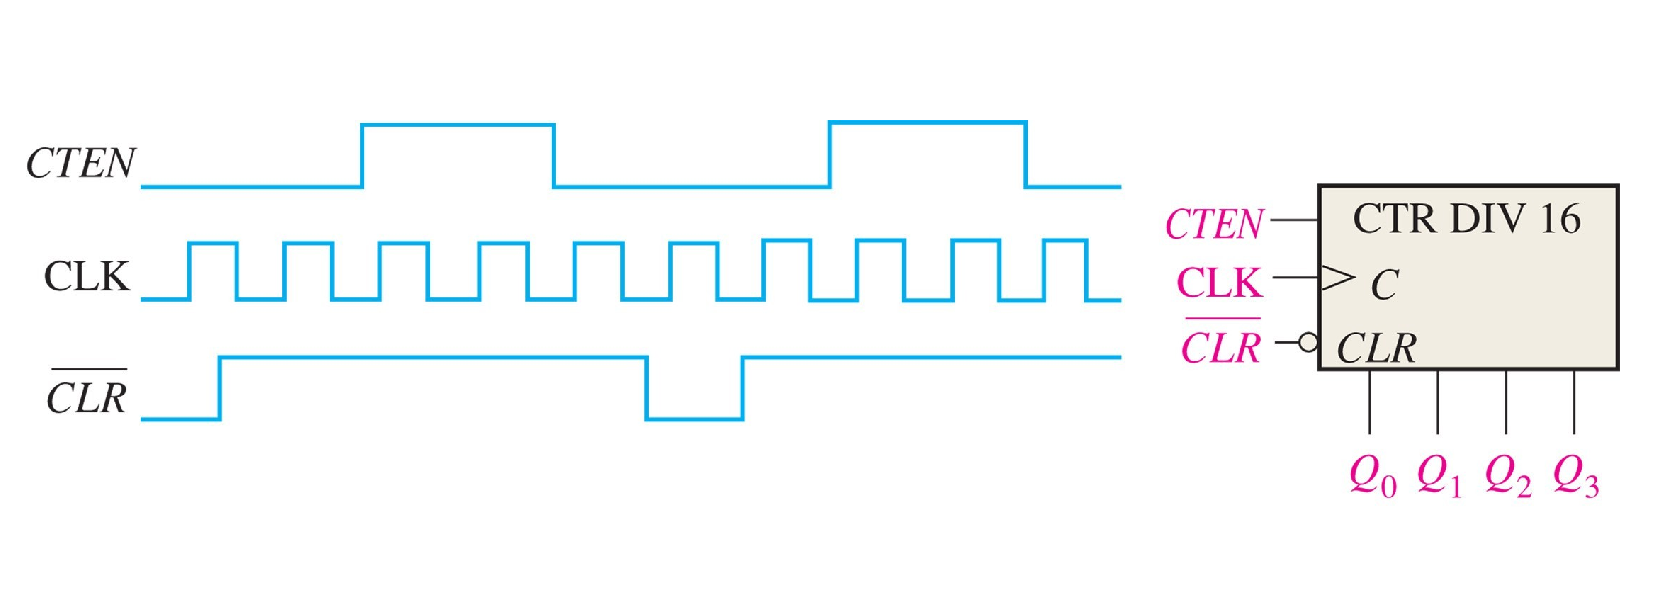
\includegraphics[width=0.8\textwidth]{figures/counter1.pdf}
\caption{\label{fig:count} A 16-state counter with enable and clear functions.}
\end{figure}
\end{enumerate}

\end{document}